\chapter{Search}

\section{Search Problems}

Searching is one of the most \itblue{fundemental techniques} in AI, underlying sub-module in many AI systems. Ai can \itblue{solve} many problems that homansare not good at, and achieve \itblue{super-human performance} in many domains (e.g. chess, go, etc.).

\begin{listu}
    \item \textbf{Benefits}

    \begin{listu}
        \item Useful as ageneral algorithmic technique for solving problems, both in AI and in other areas.

        \item Outperform humans in some areas (e.g. games). 

        \item Practical:

        \begin{listu}
            \item Many problems don't have specific algorithms for solving them.
            \item Useful in approximation (e.g., local search in optimization problems).
        \end{listu}

        \item Some critical aspects of intelligent behaviour, e.g., planning, can be cast as search.
    \end{listu}
    
    \item \textbf{Limitations}
    
    \begin{listu}
        \item Only shows how to solve the problem once we have it correctly formulated.
    \end{listu}
\end{listu}

% TODO: Planning and Scheduling Problems:

\subsection{Formalizing a Problem as a Search Problem}

\begin{listu}
    \item Necessary components
    
    \begin{listo}
        \item \bred{State Space}: A \term{state} is a representation of a \itblue{configuration} of the problem domain. The state space is the \itblue{set of all states} include in our model of the problem. 
        \item \bred{Initial State}: The starting configuration. 
        \item \bred{Goal State}: The configuration one wants to achieve. 
        \item \bred{Actions} (or State Space Transitions): Allowed changed to move from one state to another. 
    \end{listo}

    \item Optional Ingredients 
    
    \begin{listu}
        \item \itblue{Costs}: Representing the cost of moving from state to state. 
        \item \itblue{Heuristics}: Help guide the search process. 
    \end{listu}
\end{listu}

Once a search problem is formalized, there are a number of algorithms one can use to solve it. A \term{solution} is a \itblue{sequence of actions} or moves that can transform the \bred{initial state} into a \bred{goal state}. 

\begin{example}[Romania Travel]
    We want to travel in Romania from Arad to Bucharest as fast as possible. 

    \begin{center}
        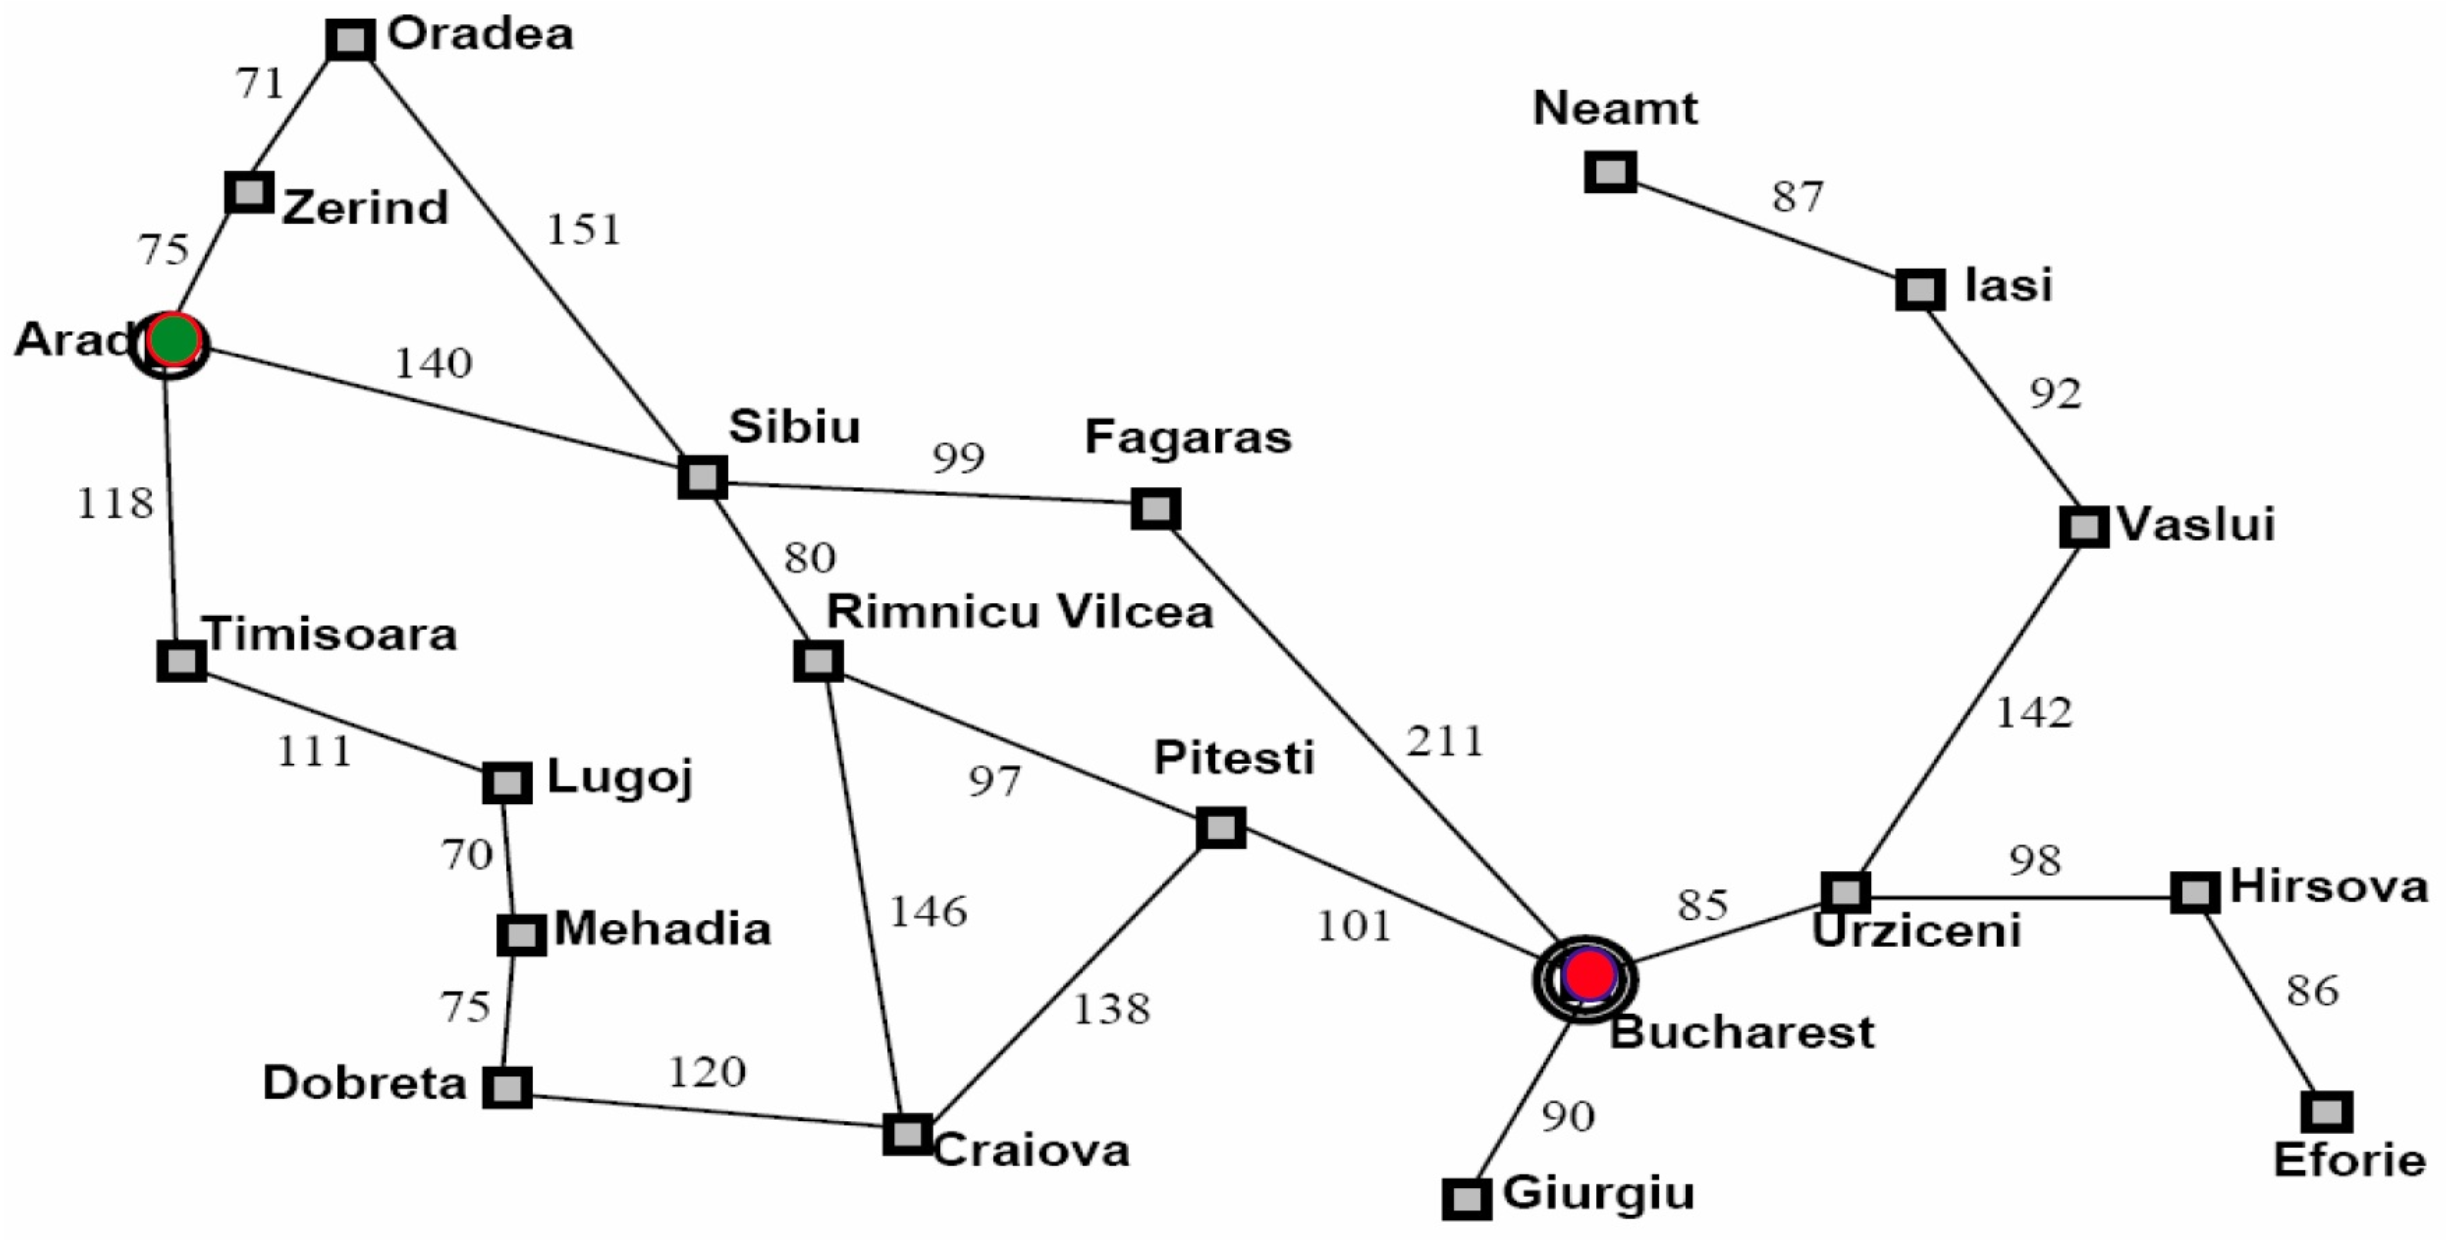
\includegraphics[width=0.75\linewidth]{figures/Romania Travel.png}
    \end{center}

    Each state would be a city. 

    \begin{listu}
        \item \bred{State Space}: The set of all cities on the map.
        \item \bred{Initial State}: Arad.
        \item \bred{Goal State}: Bucharest.
        \item \bred{Actions}: Driving between neighbouring cities.
    \end{listu}
\end{example}

\begin{example}[Water Jugs]
    We have a 3-liter jug and a 4-liter jug. We can fill either jug to the top from a tap, or we can empty either jug onto the ground. We can also pour the contents of one jug into the other until the receiving jug is full or the pouring jug is empty.

    Suppose initially the 4-liter jug is full, we want to have exactly 2 liters in the 3-liter jug.

    {~~~}

    We can use a pair of numbers to represent the state of the system: the amount of water in the 3-liter jug and the amount of water in the 4-liter jug.

    \begin{listu}
        \item \bred{State Space}: The set of all pairs of numbers $(a, b)$ where $a$ is the amount of water in the 3-liter jug and $b$ is the amount of water in the 4-liter jug.
        \item \bred{Initial State}: $(0, 4)$.
        \item \bred{Goal State}: $(2, 0)$, $(2, 1)$, $(2, 2)$, $(2, 3)$, $(2, 4)$.
        \item \bred{Actions}: 
        \begin{listu}
            \item Fill the 3-liter jug from the tap.
            \item Fill the 4-liter jug from the tap.
            \item Empty the 3-liter jug onto the ground.
            \item Empty the 4-liter jug onto the ground.
            \item Pour the contents of the 3-liter jug into the 4-liter jug.
            \item Pour the contents of the 4-liter jug into the 3-liter jug.
        \end{listu}
    \end{listu}

    \begin{remark}
        When formalizing a search problem, always consider these questions:

        \begin{listo}
            \item Can we reach all states fron any given start state?

            \item Will all actions result in a change of state? 

            \bred{No!} Imagine you have $(3, 4)$ and you try to fill the 3-liter jug from the tap. You will still have $(3, 4)$.
        \end{listo}
    \end{remark}
\end{example}

\subsubsection{More Complex Situations}

In more complex situations, 

\begin{listu}
    \item Actions may lead to \bred{multiple states}. 
    
    For example, filpping a coin may lead to heads or tails.

    \item We may not be \bred{sure of a given state}
    
    For example, when prize is behind door 1, 2, or 3.

    \item Such situations require techniques for reasoning under uncertainty: assign probabilities to given outcomes.
\end{listu}

\subsection{Graphical Representation}

\begin{center}
    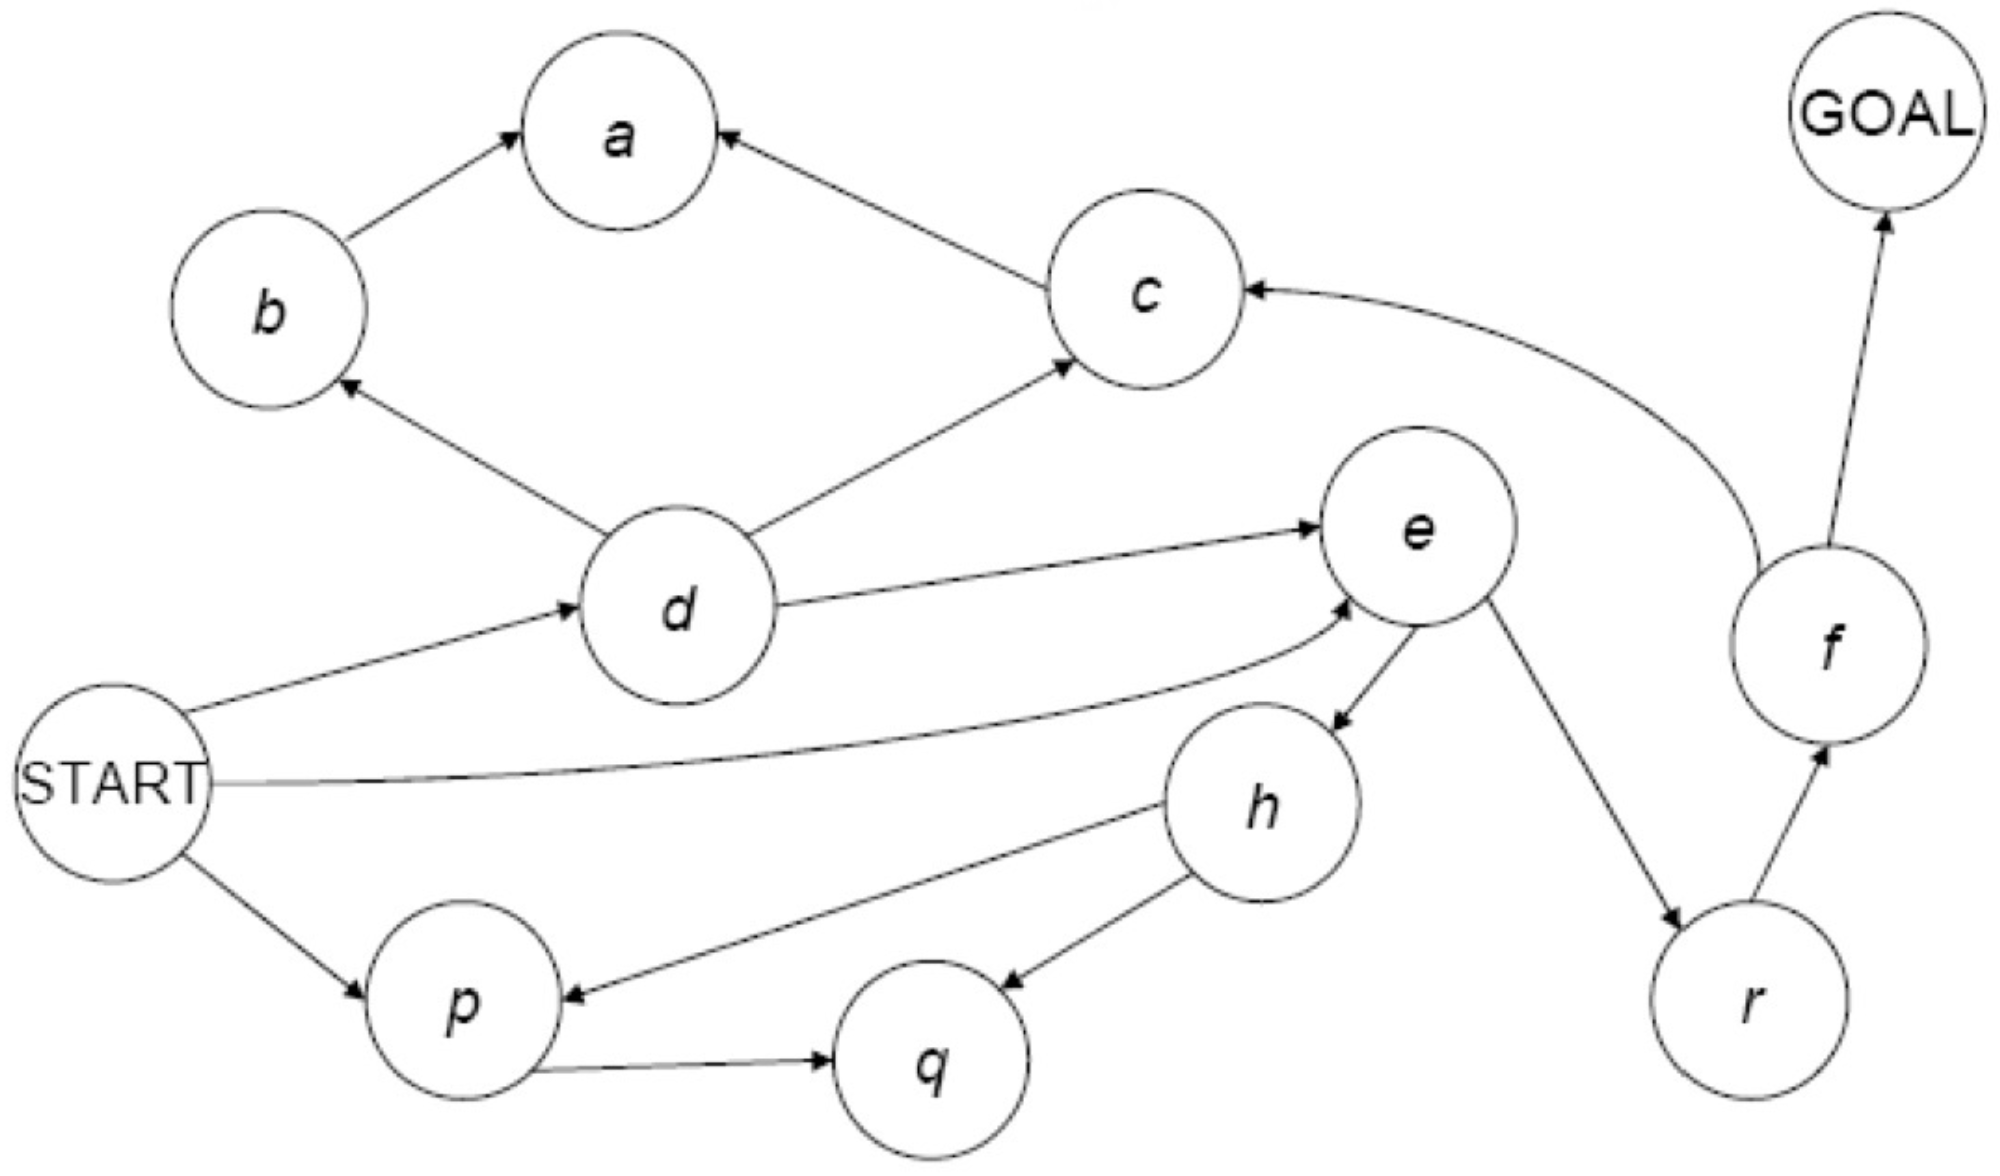
\includegraphics[width=0.67\linewidth]{figures/Search Graph Rep.png}
\end{center}

Assuming a finite search space, the

\begin{listu}
    \item \bred{vertices} represent states in the search space; and the 
    \item \bred{edges} represent transitions resulting from actions (or successor functions).
\end{listu}

\subsubsection{Search Tree}

\begin{definition}[Search Tree]
    A \term{search tree} is a \itblue{directed graph} where

    \begin{listu}
        \item Each node represents a state.
        \item Each edge represents an action.
        \item The root node represents the initial state.
        \item The leaf nodes represent goal states.
    \end{listu} 
\end{definition}

A search tree reflects the behaviour of an algorithm as it walks through a search problem. It has two important properties:

\begin{listu}
    \item \term{Solution depth}, denoted $d$, the depth of the shallowest goal node in the tree.
    \item \term{Maximum branching factor}, denoted $b$, the maximum number of children of any node in the tree.
\end{listu}

\begin{remark}
    Note that the \bred{same} state may appear \bred{multiple times} in a search tree.
\end{remark}

\begin{remark}
    It is important to distinguish between \bred{states} from \bred{nodes}. 

    \begin{listu}
        \item A \bred{state} represents a possible configuration of the world. 
        \item A \itblue{node} is a data structure constituting part of a search tree. It includes 
        \begin{listu}
            \item a \bred{state} and 
            \item the \bred{parent node}, 
            \item the \bred{action} that led to this node, and 
            \item the \bred{cost} of the path from the initial node to this node. 
        \end{listu}
        \item  Intuitively speaking, each node corresponds with a path from the initial state to the node's state.
        \item Two \bred{different nodes} are allowed to contain the \bred{same world state}.
    \end{listu}
\end{remark}

\subsection{Algorithms for Search}

\begin{listu}
    \item \textbf{Input}
    
    \begin{listu}
        \item \textbf{Initial node}

        \item \textbf{Successor Function} $S(x)$
        
        returns the set of nodes that can be reached from node $c$ via a single action. 

        \item \textbf{Goal Test Function} $G(x)$
        
        returns true if node $c$ satisfies the goal condition. 

        \item \textbf{Action Cost Function} $C(x, a, y)$
        
        returns the cost of moving from node $x$ to node $y$ using action $a$.

        Note that $C(x, a, y) = \infty$ if $y$ is not reachable from $a$ via $a$. 
    \end{listu}

    \item \textbf{Output}
    
    \begin{listu}
        \item A \itblue{sequence of actions} that transforms the initial node satisfying the goal test. 
        \item The sequence might be, \term{optimal in cost} for some algorithms, \term{optimal in length} for some algorithms, come with \bred{no optimality} guarantees from other algorithms.
    \end{listu}

    \item \textbf{Procedure}
    
    \begin{listu}
        \item Put nodes have not yet expanded in a list called the \term{\texttt{Frontier}} (or \term{Open}).
        \item Initially, only the \itblue{initial node} is in the \texttt{Frontier}.
        \item At each iteration, pull a node from the \texttt{Frontier}, apply $S(x)$, and insert the children back into the \texttt{Frontier}.
        \item Repeat until pulling a goal node.
    \end{listu}
\end{listu}

\newpage
\begin{algorithm}
    \caption{Tree Search Algorithm}
    
    \begin{algorithmic}[1]
        \Function{TreeSearch}{Frontier, Successors, Goal?}
            % If frontier is empty, return failure
            \If{Frontier is empty}
                \State \Return failure
            \EndIf

            \State Curr $\gets$ select state from frontier

            \If{Goal?(Curr)}
                \State \Return Curr
            \EndIf

            \State Frontier' $\gets$ Frontier $-$ \{ Curr \} $\cup$ Successors(Curr)

            \State \Return \Call{TreeSearch}{Frontier', Successors, Goal?}
        \EndFunction
    \end{algorithmic}
\end{algorithm}

% TODO: example

Note that the search terminates only when a goal node is expanded into the \texttt{Frontier}.